\documentclass{article}
\usepackage[a4paper,top=2.5cm,bottom=2.5cm,left=2.5cm,right=2.5cm]{geometry}
\usepackage{makeidx}
\usepackage{graphicx}
\usepackage{listings}
\usepackage{color}
\usepackage[table]{xcolor}
\usepackage{alltt}
\usepackage{ifpdf}
\ifpdf
\usepackage[pdftex,
            pagebackref=true,
            colorlinks=true,
            linkcolor=black,
            unicode
           ]{hyperref}
\else
\usepackage[ps2pdf,
            pagebackref=true,
            colorlinks=true,
            linkcolor=black,
            unicode
           ]{hyperref}
\usepackage{pspicture}
\fi
\usepackage[utf8]{inputenc}
%\usepackage{mathptmx}
\usepackage[scaled=.90]{helvet}
\usepackage{courier}
\usepackage{sectsty}
%\usepackage{amssymb}
\usepackage[titles]{tocloft}
%\usepackage{doxygen}
\lstset{language=C++,inputencoding=utf8,basicstyle=\footnotesize,breaklines=true,breakatwhitespace=true,tabsize=8,numbers=left }
\lstset{language=XML,inputencoding=utf8,basicstyle=\footnotesize,breaklines=true,breakatwhitespace=true,tabsize=8,numbers=left,keywordstyle=\color{blue},morekeywords={profile,modules,launcher},numberstyle=\tiny\color{gray}, backgroundcolor=\color{gray}}
\lstset{language=bash,inputencoding=utf8,basicstyle=\footnotesize,breaklines=true,breakatwhitespace=true,tabsize=8 }

\makeindex
\setcounter{tocdepth}{3}
%\renewcommand{\footrulewidth}{0.4pt}
\renewcommand{\familydefault}{\sfdefault}
\hfuzz=15pt
\setlength{\emergencystretch}{15pt}
\hbadness=750
\tolerance=750

\author{Sogeti High Tech}
\title{Runtime Configuration for MPC - User Manual}
\date{\today}

\begin{document}
\hypersetup{pageanchor=false,citecolor=blue}
\maketitle

\newpage
\pagenumbering{roman}
\tableofcontents
\newpage
\pagenumbering{arabic}
\hypersetup{pageanchor=true,citecolor=blue}

\section{Introduction}

Since MPC 2.4.1, a configuration system has been introduced through the module \texttt{MPC\_Config}: it enables the user to setup some parameters at the runtime when running his binary with MPC.
\newline

\noindent This manual will explain to an user how he can use and modify the configuration for running his applications with \texttt{mpcrun}.

\section {The configuration file structure}

In MPC 2.4.1, some variables can be configured during the runtime. To do this, a configuration file defines all the variables and their values, and MPC will load it at the execution.
\newline

\noindent An example of a configuration file can be found in the \texttt{\$PREFIX/share/mpc} folder, where \texttt{\$PREFIX} matches to the install directory of MPC.
\newline

\noindent The configuration file is written in XML, and two parts make up it:
\begin{enumerate}
\item A first one listing all the available profiles and their associated parameters;
\item An other one defining which profiles to apply at runtime depending on the values of environment variables.
\end{enumerate}

\section{Define a configuration file}

\subsection{Defining profiles}

In this manual, and to illustrate the configuration system, we will define two profiles: the default one and an other for debugging.

\subsubsection{Step 1: Define a default profile}

A configuration file must have a default profile (see XML just beyond): it initializes all the variables of the configuration system with their default values.

\lstset{language=XML}
\begin{lstlisting}[title=Example of \texttt{default} profile]
<profile>
  <name>default</name>
  <modules>
    <launcher>
      <nb_node>4</nb_node>
      <nb_processor>4</nb_processor>
      <share_node>false</share_node>
    </launcher>
    <allocator>
      <numa>true</numa>
      <debug>false</debug>
    </allocator>
  </modules>
<profile>
\end{lstlisting}

\noindent This simple example defines three variables for a module called \texttt{launcher}, and two for \texttt{allocator}.
\newline

\noindent The parameters inside a module can be of different types (matching to C types) :
\begin{itemize}
\item Numbers such as integers, doubles, etc.;
\item String;
\item Size (i.e. \texttt{50 MB}, \texttt{10 PB}, etc.);
\item Boolean (\texttt{true} or \texttt{false});
\item Enum;
\item Function Pointer.
\end{itemize}

\noindent All the parametrizable variables can be listed by executing the command \texttt{man mpc\_config}: it gives information (type, default value, description) for each variable.

\subsubsection{Step 2: Define a profile for debugging}

To debugging applications, some parameters need to be initialized with different values than the default profile ones. So the user can defined a new profile as beyond:

\lstset{language=XML}
\begin{lstlisting}[title=Example of \texttt{debug} profile]
<profile>
  <name>debug</name>
  <modules>
    <launcher>
      <nb_node>2</nb_node>
      <nb_processor>2</nb_processor>
    </launcher>
    <allocator>
      <debug>true</debug>
    </allocator>
  </modules>
<profile>
\end{lstlisting}

\noindent While the default profile must have \texttt{default} as name, the name of this new profile has no importance: to be coherent with our example, we call it \texttt{debug}. Selecting this profile will overwrite the default values with those ones.

\subsection{Mapping profiles}

One way to select the profiles to apply during execution is to define mapping in the configuration file. The XML code beyond will enable the user to select the \texttt{debug} profile depending on the value of the environment variable \texttt{MPC\_DEBUG}.

\lstset{language=XML}
\begin{lstlisting}[title=Example of mapping to apply \texttt{debug} profile]
<mapping>
  <selectors>
    <env name=''MPC_DEBUG''>true</env>
  </selectors>
  <profiles>
    <profile>debug</profile>
  </profiles>
<mapping>
\end{lstlisting}

\noindent The user can define multiple mappings which will be surrounded with \texttt{<mappings>...</mappings>}. By default, the \texttt{default} profile is applied which means that if the user does not defined any mapping, the variables into the configuration will be initialized.

\section{Configuration test}

MPC will use many configuration files that it will apply in the following order:
\begin{enumerate}
\item \texttt{\$PREFIX/share/mpc/config.xml};
\item \texttt{\$PREFIX/share/mpc/config.xml.example} if the previous file does not exist;
\item the file given by the parameter \texttt{--config} of \texttt{mpcrun} if present.
\end{enumerate}

\noindent As an example, let's assume an executable called \texttt{test}: its goal is to simply print the values of the variables which are in the configuration system.

\subsection{Simple execution without parameters}

If the binary \texttt{test} is simply called executing the command \texttt{./test}, the ouput is:

\lstset{language=bash}
\begin{lstlisting}[title=Output of a simple execution]
launcher:
    nb_node: 4
    nb_processor: 4
    share_node: false

allocator:
    numa: true
    debug: false
\end{lstlisting}

\noindent If nothing is precised, the \texttt{default} profile will be loaded at execution.

\subsection{Execution in debugging mode}

\subsubsection{Using the environment variable MPC\_DEBUG}
\label{conf_debug_mode}

If the user executes the command \texttt{MPC\_DEBUG=true ./test}, this will enable the \texttt{debug} profile:
\begin{enumerate}
\item the values of the \texttt{default} are first loaded;
\item all the variables redefined in the \texttt{debug} profile are overwritten, and all the others keep their previous values.
\end{enumerate}

\noindent The output of this command is:

\lstset{language=bash}
\begin{lstlisting}[title=Output when enabling the debug mode]
launcher:
    nb_node: 2
    nb_processor: 2
    share_node: false

allocator:
    numa: true
    debug: true
\end{lstlisting}

\subsubsection{Using the option --profiles of mpcrun}

The user can also precise the profiles he wants to apply using the option \texttt{--profiles} of \texttt{mpcrun}.
\newline

\noindent The command \texttt{mpcrun --profiles=debug ./test} produces the same output as in §\ref{conf_debug_mode}.

\subsubsection{Using the environment variable MPC\_USER\_PROFILE}

The user can also precise the profiles he wants to apply using the environment variable \texttt{MPC\_USER\_PROFILE}.
\newline

\noindent The command \texttt{MPC\_USER\_PROFILE=debug ./test} produces the same output as in §\ref{conf_debug_mode}.

\subsection{Simple execution with parameters}

If an argument is passed to the executable, it will overwrite the values put in configuration for the associated variable. For example, if the argument \texttt{-n=3} sets the number of nodes, the command \texttt{./test -n=3} outputs:

\lstset{language=bash}
\begin{lstlisting}[title=Simple execution with parameters]
launcher:
    nb_node: 3
    nb_processor: 2
    share_node: false

allocator:
    numa: true
    debug: false
\end{lstlisting}

\section{Network configuration}

The network that will be used during the execution can also be parametrized into the configuration file between the tags \texttt{<networks>...</networks>}. For the moment, MPC 2.5.0 only supports Infiniband and TCP.
\newline

\noindent The first step is to defined all the network configurations available:

\lstset{language=XML}
\begin{lstlisting}[title=Define network configurations]
<configs>
  <config>
    <name>ib1</name>
    <driver>
      <infiniband>
        <param1>4</param1>
        <param2>300</param>
      </infiniband>
    </driver>
  </config>
  <config>
    <name>ib2</name>
    <driver>
      <infiniband>
        <param1>2</param1>
        <param2>1500</param>
      </infiniband>
    </driver>
  </config>
  <config>
    <name>tcp1</name>
    <driver>
      <tcp>
        <fake_param>0</fake_param>
      </tcp>
    </driver>
  </config>
</configs>
\end{lstlisting}

\noindent Next step is to defined the different rails which will use the previous network configurations. A rail consists in a specific topology to use, and one of the defined configurations.

\lstset{language=XML}
\begin{lstlisting}[title=Define network configurations]
<rails>
  <rail>
    <name>rail_ib1</name>
    <device>0</device>
    <topology>ondemand</topology>
    <config>ib1</config>
  </rail>
  <rail>
    <name>rail_ib2</name>
    <device>0</device>
    <topology>fully</topology>
    <config>1500</config>
  </rail>
  <rail>
    <name>rail_itcp1</name>
    <device>0</device>
    <topology>fully</topology>
    <config>tcp1</config>
  </rail>
</rails>
\end{lstlisting}

\noindent The final step is to defined the different options that the user can choose with the option \texttt{--net} of \texttt{mpcrun}.

\lstset{language=XML}
\begin{lstlisting}[title=Define network modes]
<cli_options>
  <cli_option>
    <name>ib</name>
    <rails>
      <rail>rail_ib1</rail>
    </rails>
  </cli_option>
  <cli_option>
    <name>tcp</name>
    <rails>
      <rail>rail_tcp1</rail>
    </rails>
  </cli_option>
  <cli_option>
    <name>tcpoib</name>
    <rails>
      <rail>rail_ib1</rail>
      <rail>rail_ib2</rail>
    </rails>
  </cli_option>
</cli_options>
\end{lstlisting}

\noindent The configuration system allow the user to define multirail by selecting many rails for a network mode. Using the previous code, the options for the option \texttt{--net} are \texttt{ib}, \texttt{ib} and \texttt{tcpoib}.
\newpage

\section{The configuration editor}

The figure \ref{fig:empty_editor} shows the editor interface as the user will see it at launching.

\begin{figure}[!h]
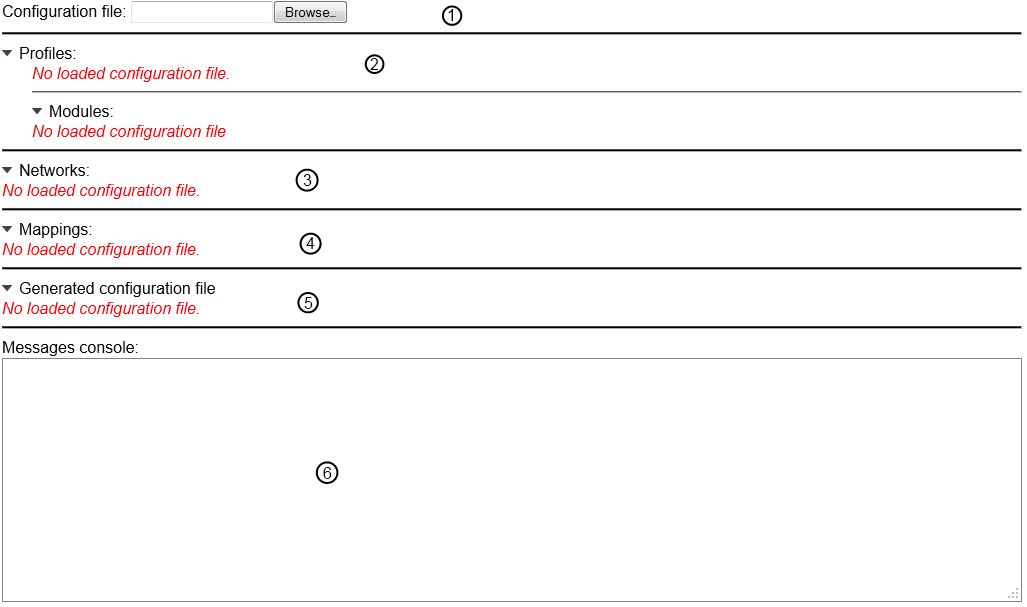
\includegraphics[width=\textwidth]{./pictures/empty_editor.png}
\caption{Editor interface at launching}
\label{fig:empty_editor}
\end{figure}

\noindent The interface is divided in several parts:
\begin{enumerate}
\item Loading of an XML configuration file;
\item Profiles displaying (modules);
\item Networks displaying;
\item Mappings displaying;
\item XML file generated from data of the previous sections;
\item Messages console (Info, Warning, Error).
\end{enumerate}

\subsection{Profiles displaying}

The figure \ref{fig:modules_editor} shows the profiles section once a configuration file loaded.

\begin{figure}[!h]
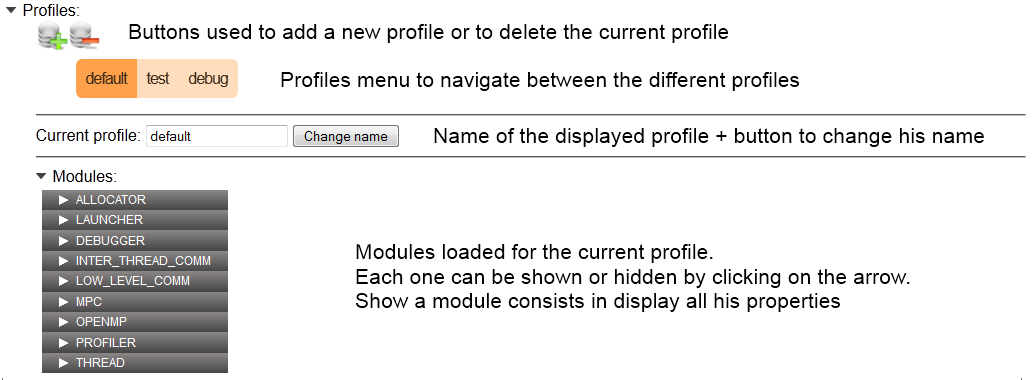
\includegraphics[width=\textwidth]{./pictures/modules_editor.png}
\caption{Profile display}
\label{fig:modules_editor}
\end{figure}

\noindent Two buttons let the user to add or delete a profile (in case of deletion, the activated profile will be erased).
\newline

\noindent A menu let the user to switch between all the available profiles.
\newline

\noindent A input of text type displays the name of the activated profile. This field lets the user to rename a profile (the ``default'' profile cannot be renamed).
\newline

\noindent The ``modules'' part displays the modules and their asociated properties (see figure \ref{fig:module_editor}).

\begin{figure}[!h]{c}
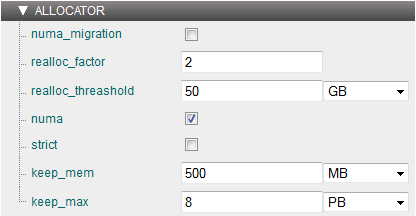
\includegraphics{./pictures/module.png}
\caption{Module display}
\label{fig:module_editor}
\end{figure}

\noindent To help the user who wants to change a property value, a tooltip is associated to each field (see figure \ref{fig:title_editor}: it describes this property, and gives the original default value.

\begin{figure}[!h]
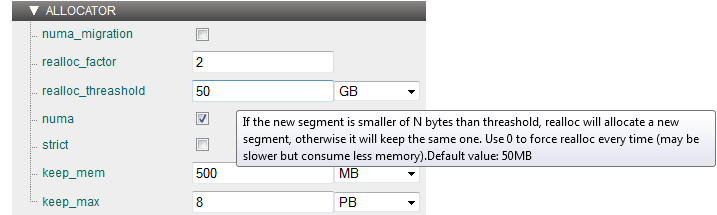
\includegraphics[width=\textwidth]{./pictures/title_editor.png}
\caption{Tooltip for the 'realloc\_threshold' property}
\label{fig:title_editor}
\end{figure}

\subsection{Networks displaying}

The figure \ref{fig:networks_editor} shows the networks section once a configuration file loaded. The menu (1) lists all the networks options:
\begin{itemize}
\item ``CLI options'' is the list of all the available values for the \texttt{-net} option of \texttt{mpcrun};
\item ``Rails'' is the list of all the available rails;
\item ``Drivers'' is the list of all the available drivers.
\end{itemize}

\noindent The editor let the user to add or delete any network option.

\begin{figure}[!h]
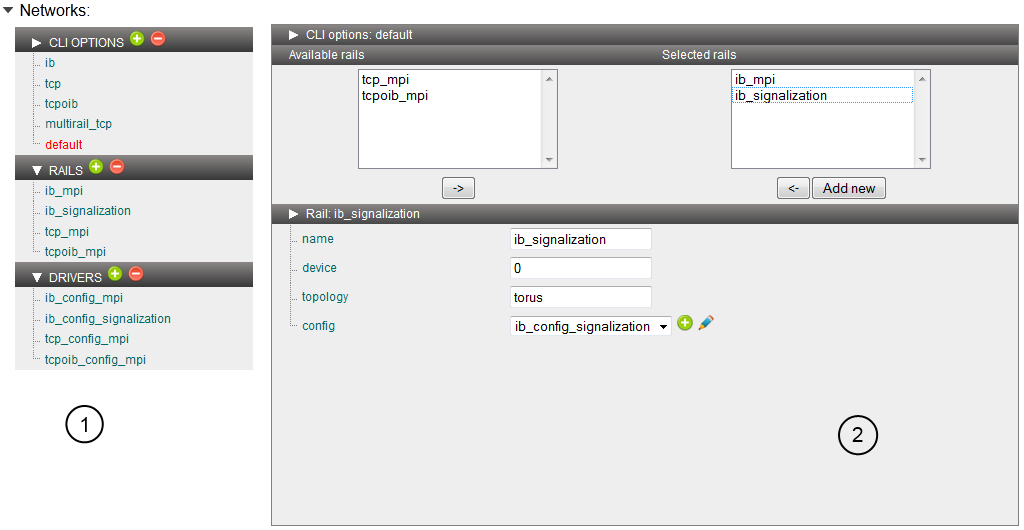
\includegraphics[width=\textwidth]{./pictures/networks_editor.png}
\caption{Networks display}
\label{fig:networks_editor}
\end{figure}

\noindent The properties of a given option are displayed in the right part after a double click on the item. The figure \ref{fig:networks_editor} shows the properties for the ``default'' CLI option and the rail named ``ib\_signalization''.

\subsection{Mappings displaying}

The figure \ref{fig:mappings_editor} shows the mappings section once a configuration file loaded.

\begin{figure}[!h]
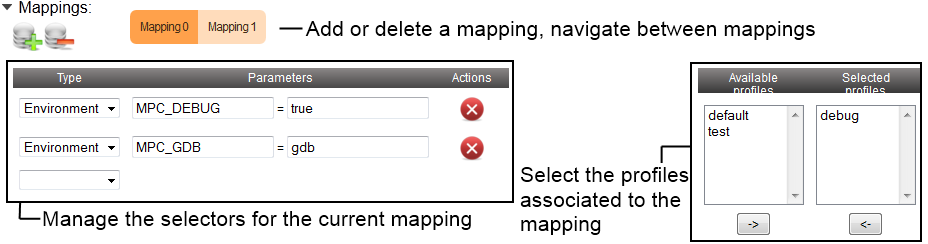
\includegraphics[width=\textwidth]{./pictures/mappings_editor.png}
\caption{Mappings display}
\label{fig:mappings_editor}
\end{figure}

\noindent As for the profiles section, two buttons let the user to add or delete a mapping. Navigation between the different mappings is done within the menu.
\newline

\noindent The table on the left side of the picture lists all the defined selectors for the current mapping. It is also possible to add or delete a given selector. The other table lists all the profiles that will be loaded if all the selectors are checked.

\subsection{The XML generated file}

The figure \ref{fig:generated_editor} shows the result of the generation of a new XML configuration file using data of the sections ``profiles'', ``networks'' and ``mappings''. The XML code cannot be directly modified through this element. The saving button let the user to save the file on a local storage: if the generated file does not match to the associated XSD, the saving will be impossible.

\begin{figure}[!h]
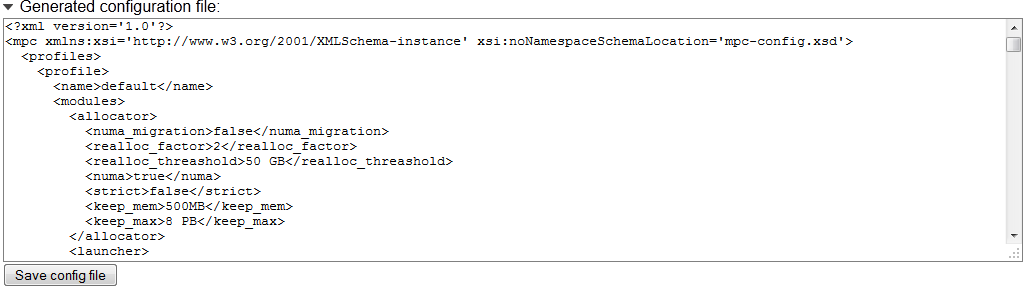
\includegraphics[width=\textwidth]{./pictures/generated_editor.png}
\caption{XML generated display}
\label{fig:generated_editor}
\end{figure}

\subsection{Messages console}

The figure \ref{fig:messages_editor} shows the console displaying all the messages (Info, Error, Warning) producing by the editor.

\begin{figure}[!h]
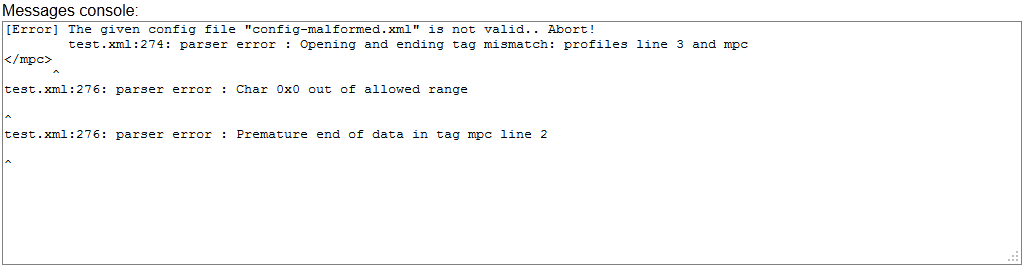
\includegraphics[width=\textwidth]{./pictures/messages_editor.png}
\caption{Messages console}
\label{fig:messages_editor}
\end{figure}

\newpage

\section{Helpful commands}

\subsection{mpc\_print\_config}

\texttt{mpc\_print\_config} is a small executable that prints the configuration in different ways:
\begin{itemize}
\item XML mode:
\lstset{language=XML}
\begin{lstlisting}
<profile>
  <name>default</name>
  <modules>
    <launcher>
      <nb_node>4</nb_node>
      <nb_processor>4</nb_processor>
      <share_node>false</share_node>
    </launcher>
    <allocator>
      <numa>true</numa>
      <debug>false</debug>
    </allocator>
  </modules>
<profile>
\end{lstlisting}
\item text mode:
\lstset{language=bash}
\begin{lstlisting}
config:
    modules:
        launcher:
            nb_node: 4
            nb_processor: 4
            share_node: false

        allocator:
            numa: true
            debug: false
\end{lstlisting}
\end{itemize}

\noindent To get more information, execute \texttt{mpc\_print\_config --help}.

\subsection{mpc\_edit\_config}

\texttt{mpc\_edit\_config} is a small executable that opens the editor. By default, the editor is opened with the first \texttt{firefox} founded in the user PATH. However, the option \texttt{-b} or \texttt{--browser} can be used to specify an other browser.

\end{document}
